%%%%%%%%%%%%%%%%%%%%%%%%%%%%%%%%%%%%%%%%%%%%%%%%%%%%%%%%%%%%%%%%%%%%%%%%%%%%%%%%%%
\begin{frame}[fragile]\frametitle{}
\begin{center}
{\Large Agentic RAG using LlamaIndex}
\end{center}
\end{frame}


%%%%%%%%%%%%%%%%%%%%%%%%%%%%%%%%%%%%%%%%%%%%%%%%%%%%%%%%%%%
\begin{frame}[fragile]\frametitle{LlamaIndex: Components and Architecture}
\begin{columns}
    \begin{column}[T]{0.6\linewidth}
      \begin{itemize}
		\item Components: Data connectors, indices, LLM interfaces, and parsers
		\item Tools: Interfaces for vector databases, web search, calculators, and APIs
		\item Agents: Autonomous reasoning entities using LLMs for decision making
		\item Workflows: Event-driven orchestration for complex multi-agent processes
		\item Modular Design: Plug-and-play architecture with swappable components
		\item LlamaHub Integration: 40+ pre-built tools and community connectors
	  \end{itemize}
    \end{column}
    \begin{column}[T]{0.4\linewidth}
		\begin{center}
		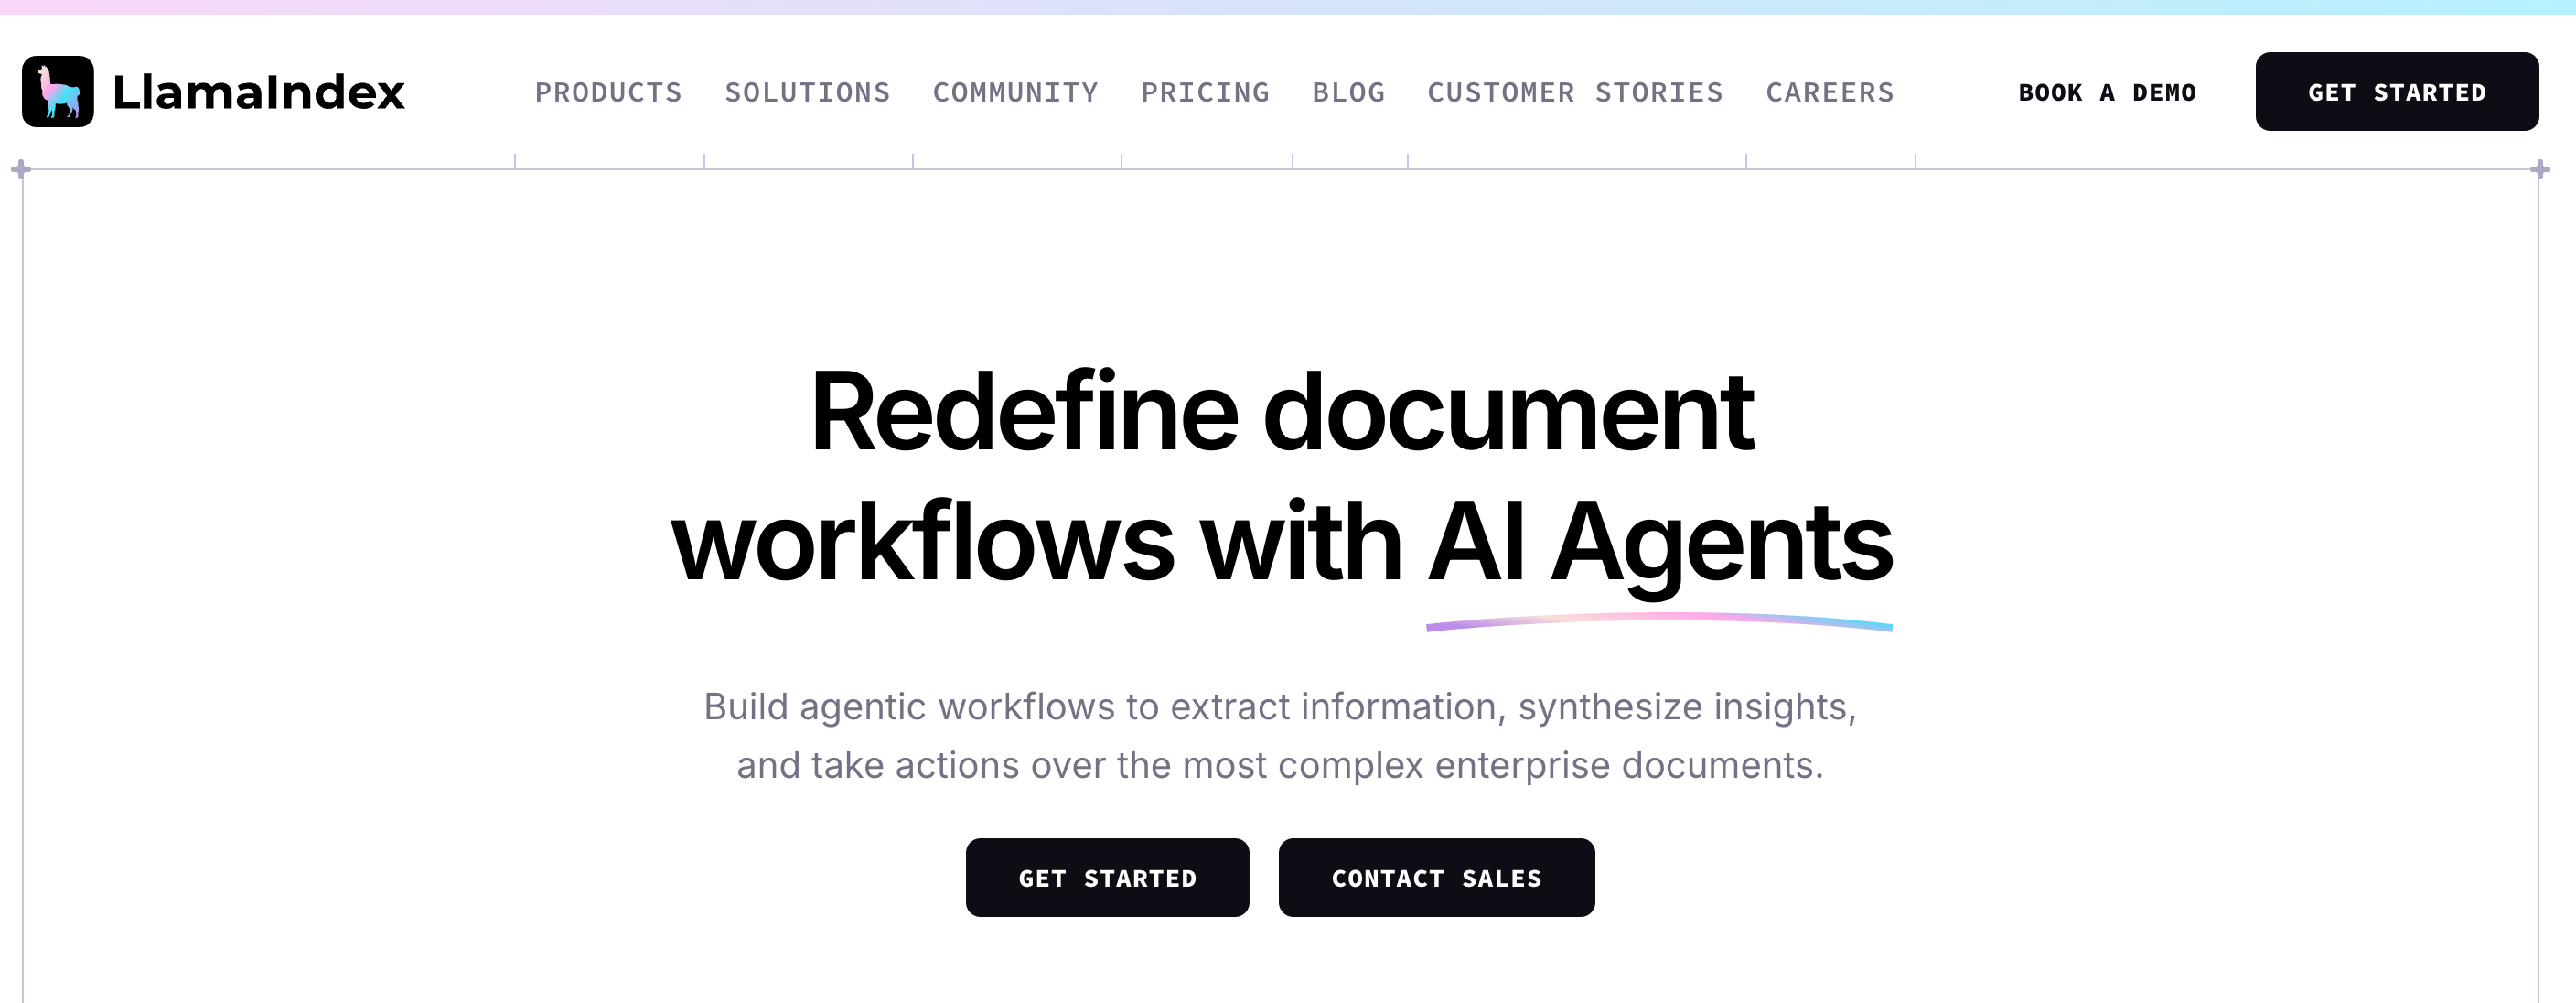
\includegraphics[width=0.8\linewidth,keepaspectratio]{aiagents58}
		
		{\tiny (Ref: Vizuara AI Agents Bootcamp)}
		
		\end{center}	
    \end{column}
  \end{columns}
\end{frame}

%%%%%%%%%%%%%%%%%%%%%%%%%%%%%%%%%%%%%%%%%%%%%%%%%%%%%%%%%%%
\begin{frame}[fragile]\frametitle{LlamaIndex: Unique Features}
\begin{columns}
    \begin{column}[T]{0.6\linewidth}
      \begin{itemize}
		\item Clear Workflow System: Structured agent pipelines with state management
		\item LlamaParse: GenAI-native document parsing for PDFs and complex files
		\item LlamaHub Tools: Ready-to-use connectors for Google Drive, Slack, search engines
		\item Plug-and-Play Components: Lego-like assembly of vector stores and LLM connectors
		\item Advanced Document Processing: Intelligent parsing for optimal LLM consumption
		\item One-Stop Framework: Complete toolkit beyond just retrieval or prompting
	  \end{itemize}
    \end{column}
    \begin{column}[T]{0.4\linewidth}
		\begin{center}
		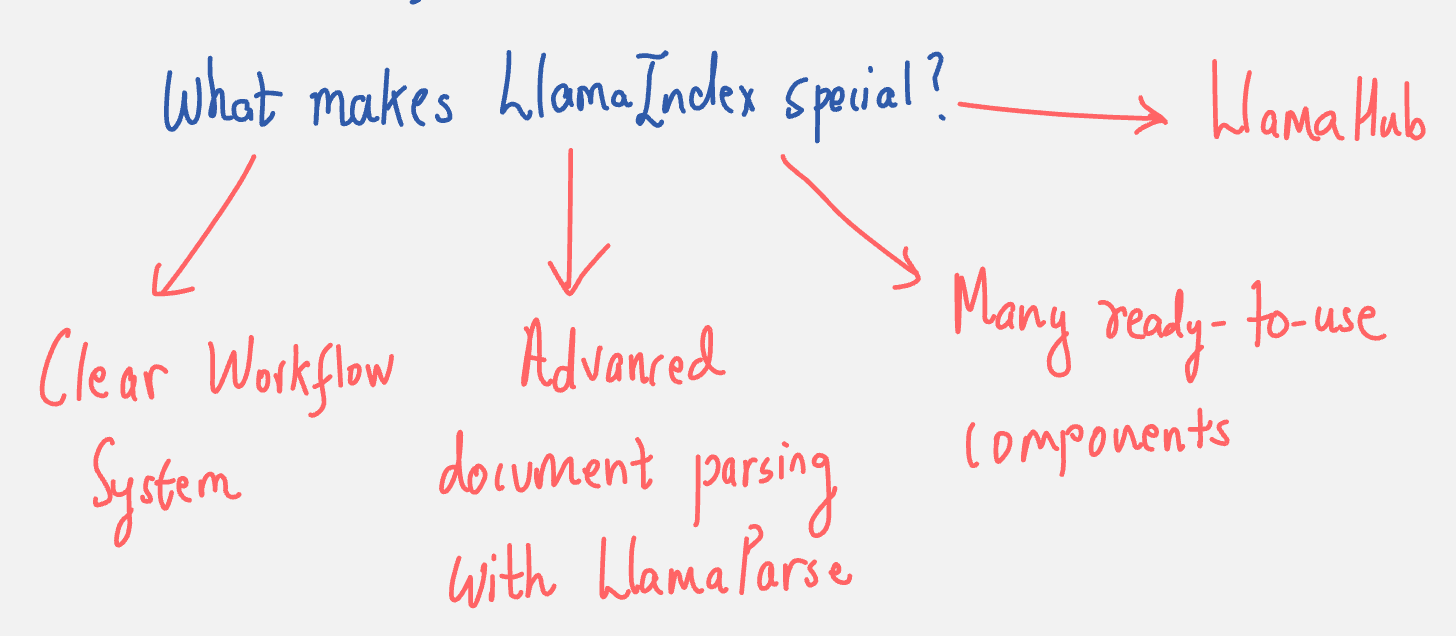
\includegraphics[width=0.8\linewidth,keepaspectratio]{aiagents59}
		
		{\tiny (Ref: Vizuara AI Agents Bootcamp)}
		\end{center}	
    \end{column}
  \end{columns}
\end{frame}


%%%%%%%%%%%%%%%%%%%%%%%%%%%%%%%%%%%%%%%%%%%%%%%%%%%%%%%%%%%
\begin{frame}[fragile]\frametitle{Agentic RAG Implementation: Data Setup}

      \begin{itemize}
		\item Document Loading: SimpleDirectoryReader for PDF and text files
		\item Text Chunking: SentenceSplitter with configurable chunk sizes (1024 tokens)
		\item LLM Configuration: OpenAI GPT-3.5-turbo for reasoning and generation
		\item Embedding Setup: OpenAI text-embedding-ada-002 for vector similarity
		\item Multiple Index Creation: Vector index for specific facts, Summary index for overviews
		\item Query Engine Setup: Specialized engines for different retrieval strategies
	  \end{itemize}


\end{frame}

%%%%%%%%%%%%%%%%%%%%%%%%%%%%%%%%%%%%%%%%%%%%%%%%%%%%%%%%%%%
\begin{frame}[fragile]\frametitle{Step 1: Loading and Chunking Data}


		\begin{lstlisting}
from llama_index.core import SimpleDirectoryReader, SentenceSplitter

# Load the document
reader = SimpleDirectoryReader(input_files=["State_of_AI_2025.pdf"])
documents = reader.load_data()
print(f"Loaded {len(documents)} document(s).")

# Split document into nodes (chunks)
splitter = SentenceSplitter(chunk_size=1024)
nodes = splitter.get_nodes_from_documents(documents)
print(f"Produced {len(nodes)} text chunks.")
		\end{lstlisting}	

\end{frame}

%%%%%%%%%%%%%%%%%%%%%%%%%%%%%%%%%%%%%%%%%%%%%%%%%%%%%%%%%%%
\begin{frame}[fragile]\frametitle{Step 2: Configuring LLM and Embeddings}


		\begin{lstlisting}
from llama_index.core import Settings
from llama_index.llms.openai import OpenAI
from llama_index.embeddings.openai import OpenAIEmbedding

Settings.llm = OpenAI(model="gpt-3.5-turbo")
Settings.embed_model = OpenAIEmbedding(model="text-embedding-ada-002")
		\end{lstlisting}	

\end{frame}


%%%%%%%%%%%%%%%%%%%%%%%%%%%%%%%%%%%%%%%%%%%%%%%%%%%%%%%%%%%
\begin{frame}[fragile]\frametitle{Step 3: Creating Multiple Indexes}


		\begin{lstlisting}
from llama_index.core import VectorStoreIndex, SummaryIndex

# Create a summary index (for high-level overview)
summary_index = SummaryIndex(nodes)

# Create a vector store index (for semantic search)
vector_index = VectorStoreIndex(nodes)
		\end{lstlisting}	

\end{frame}

%%%%%%%%%%%%%%%%%%%%%%%%%%%%%%%%%%%%%%%%%%%%%%%%%%%%%%%%%%%
\begin{frame}[fragile]\frametitle{Step 4: Building Query Engines}


		\begin{lstlisting}
# Create a query engine for each index
summary_query_engine = summary_index.as_query_engine(response_mode="tree_summarize")
vector_query_engine = vector_index.as_query_engine()
		\end{lstlisting}	

\end{frame}

%%%%%%%%%%%%%%%%%%%%%%%%%%%%%%%%%%%%%%%%%%%%%%%%%%%%%%%%%%%
\begin{frame}[fragile]\frametitle{Step 5: Wrapping Query Engines as Tools}


		\begin{lstlisting}
from llama_index.core.tools import QueryEngineTool

# Create tool interfaces for each query engine
summary_tool = QueryEngineTool.from_defaults(
    query_engine=summary_query_engine,
    description="Useful for summarizing the State of AI 2025 report."
)
vector_tool = QueryEngineTool.from_defaults(
    query_engine=vector_query_engine,
    description="Useful for retrieving specific details from the State of AI 2025 report."
)
		\end{lstlisting}	

\end{frame}

%%%%%%%%%%%%%%%%%%%%%%%%%%%%%%%%%%%%%%%%%%%%%%%%%%%%%%%%%%%
\begin{frame}[fragile]\frametitle{Step 6: Setting Up a Router Query Engine}


		\begin{lstlisting}
from llama_index.core.query_engine.router_query_engine import RouterQueryEngine
from llama_index.core.selectors import LLMSingleSelector

# Create a router that can select between the two query engine tools
router_engine = RouterQueryEngine(
    selector=LLMSingleSelector.from_defaults(),
    query_engine_tools=[summary_tool, vector_tool],
    verbose=True
)

response = router_engine.query("Who is Lareina Yee according to the document?")
print(response)
# (It should retrieve context and answer that Lareina Yee is one of the authors.)
		\end{lstlisting}	

\end{frame}



%%%%%%%%%%%%%%%%%%%%%%%%%%%%%%%%%%%%%%%%%%%%%%%%%%%%%%%%%%%
\begin{frame}[fragile]\frametitle{Tool Creation and Agent Setup}

      \begin{itemize}
		\item QueryEngineTool Wrapping: Convert query engines into agent-usable tools
		\item Tool Descriptions: Clear descriptions help agent choose appropriate tool
		\item RouterQueryEngine: Automated routing between summary and vector tools
		\item LLMSingleSelector: Intelligent tool selection based on query analysis
		\item AgentWorkflow: High-level API for creating agents with tool access
		\item System Prompts: Context-aware prompts for specialized agent behavior
	  \end{itemize}
  
\end{frame}

%%%%%%%%%%%%%%%%%%%%%%%%%%%%%%%%%%%%%%%%%%%%%%%%%%%%%%%%%%%
\begin{frame}[fragile]\frametitle{Step 7: Defining the Agent}


		\begin{lstlisting}
from llama_index.core.agent.workflow import AgentWorkflow

# Wrap the router query engine as a tool for the agent
assistant_tool = QueryEngineTool.from_defaults(
    query_engine=router_engine,
    name="state_of_ai_report_assistant",
    description="Tool to answer questions using the McKinsey 2025 State of AI report."
)

# Initialize the agent with this tool
agent = AgentWorkflow.from_tools_or_functions(
    tools_or_functions=[assistant_tool],
    llm=Settings.llm,
    system_prompt="You are an AI assistant skilled in answering questions about the 2025 State of AI report."
)
		\end{lstlisting}	

\end{frame}

%%%%%%%%%%%%%%%%%%%%%%%%%%%%%%%%%%%%%%%%%%%%%%%%%%%%%%%%%%%
\begin{frame}[fragile]\frametitle{Step 8: Running the Agent}


		\begin{lstlisting}
# Ask the agent a complex question
question = "Summarize the key trends in AI adoption and mention the percentage of companies using AI."
response = await agent.run(question)
print(response)
		\end{lstlisting}	

\end{frame}
